%
% Complete documentation on the extended LaTeX markup used for Insight
% documentation is available in ``Documenting Insight'', which is part
% of the standard documentation for Insight.  It may be found online
% at:
%
%     http://www.itk.org/

\documentclass{InsightArticle}

\usepackage[dvips]{graphicx}
%\usepackage{listing}						
\usepackage{listings}	
\usepackage{wrapfig}
\usepackage{amssymb,amsmath}
\usepackage{multirow,booktabs,array}
\usepackage{listings}
\usepackage{color}
				
%%%%%%%%%%%%%%%%%%%%%%%%%%%%%%%%%%%%%%%%%%%%%%%%%%%%%%%%%%%%%%%%%%
%
%  hyperref should be the last package to be loaded.
%
%%%%%%%%%%%%%%%%%%%%%%%%%%%%%%%%%%%%%%%%%%%%%%%%%%%%%%%%%%%%%%%%%%
\usepackage[
bookmarks,
bookmarksopen,
backref,
colorlinks,linkcolor={blue},citecolor={blue},urlcolor={blue},
]{hyperref}




\graphicspath{{./Figures/}}
\newcommand{\fv}{\mbox{\boldmath $f$}}
\newcommand{\Iv}{\mbox{\boldmath $I$}}
\newcommand{\xv}{\mbox{\boldmath $x$}}
\newcommand{\velocity}{\mbox{\boldmath $v$}}
\newcommand{\velocityinv}{\mbox{\boldmath $v$}^{-1}}
\newcommand{\Velocityinv}{\mbox{\boldmath $V$}^{-1}}
\newcommand{\Velocity}{\mbox{\boldmath $V$}}
\newcommand{\welocity}{\mbox{\boldmath $w$}}
\newcommand{\spatialimagegradient}{\mbox{\boldmath $I$}\mbox{$_{x}$}}
\newcommand{\perpspatialimagegradient}{\mbox{\boldmath $I$}\mbox{$^{\perp}_{x}$}}
\newcommand{\temporalimagederivative}{\mbox{$I_t$}}
\newcommand{\finitestrain}{\mbox{\boldmath $\varepsilon^{\ast}$}}
\newcommand{\smallstrain}{\mbox{\boldmath $\varepsilon$}}
\newcommand{\dispgradient}{{\bf \nabla \displace}}
\newcommand{\displace}{{\bf u}} 
\newcommand{\Id}{\text{\bf Id}}
\newcommand{\ode}{{\em O.D.E.}}
\newcommand{\odes}{{\em O.D.E.}s}
\newcommand{\G}{\mathcal{G}}
\newcommand{\J}{\mathcal{J}}
\newcommand{\phiinv}{\phi^{-1}}
\newcommand{\psiinv}{\psi^{-1}}
\newcommand{\dM}{DM}
\newcommand{\DM}{Diffeomorphometry}
\newcommand{\diff}{diffeomorphism}
\newcommand{\Diff}{Diffeomorphism}
\newcommand{\orbit}{\mathcal{O}}
\newcommand{\avg}{\mathcal{A}}
\newcommand{\avgn}{\mathcal{A}_n}
\newcommand{\avgna}{\mathcal{A}^a_{n}}
\newcommand{\nset}{\{ J_i \}_n}
\newcommand{\bari}{\bar{I}}
\newcommand{\bart}{\bar{t}}
\newcommand{\jac}{\mathcal{J}}
\newcommand{\pert}{\mbox{\boldmath $w$}}
\newcommand{\barpert}{\bar{\mbox{\boldmath $w$}}}
\newcommand{\half}{0.5}

\newcommand{\X}{{\bf X}}
\newcommand{\x}{{\bf x}}
\newcommand{\Z}{{\bf Z}}
\newcommand{\z}{{\bf z}}
\newcommand{\p}{{\bf p}}
\newcommand{\Y}{{\bf Y}}
\newcommand{\y}{{\bf y}}
\newcommand{\disp}{{\bf u}}
\newcommand{\ytild}{\tilde{{\bf y}}}
\newcommand{\q}{{\bf q}}
\newcommand{\surf}{\mathcal{S}}
\newcommand{\phij}{\phi_{ij}}
\newcommand{\aphij}{\bar{\phi}_{j}}
\newcommand{\apsij}{\bar{\psi}_{j}}
\newcommand{\aphi}{\bar{\phi}}
\newcommand{\aphiinv}{\bar{\phi}^{-1}}

\newcommand{\domain}{\Omega}
\newcommand{\meanshape}{\bf \bar{x}}
\newcommand{\g}{\mbox{\boldmath $g$}}
\newcommand{\h}{\mbox{\boldmath $h$}}
\newcommand{\yv}{\mbox{\boldmath $y$}}

\newcommand{\group}{Diff}


\newcommand{\evol}{{E_{\text{Vol}}}}
\newcommand{\epair}{{E_{\text{Pair}}}}
\newcommand{\esec}{{E_{S}}}
\newcommand{\inv}{^{-1}}
\newcommand{\vinit}{ \velocity^0_{ij}(\x,\tau=0) }
\newcommand{\avinit}{ \bar{\velocity}^0_{j}(\x,t) }
\newcommand{\avinitz}{ \bar{\velocity}^0_{j}(\x,t_a) }
\newcommand{\gz}{\nabla_{\z}}


 
\definecolor{dkgreen}{rgb}{0,0.6,0}
\definecolor{gray}{rgb}{0.5,0.5,0.5}
\definecolor{mauve}{rgb}{0.58,0,0.82}

\lstset{ %
  language=bash,                % the language of the code
  basicstyle=\footnotesize,           % the size of the fonts that are used for the code
  numbers=left,                   % where to put the line-numbers
  numberstyle=\tiny\color{gray},  % the style that is used for the line-numbers
  stepnumber=2,                   % the step between two line-numbers. If it's 1, each line 
                                  % will be numbered
  numbersep=5pt,                  % how far the line-numbers are from the code
  backgroundcolor=\color{white},      % choose the background color. You must add \usepackage{color}
  showspaces=false,               % show spaces adding particular underscores
  showstringspaces=false,         % underline spaces within strings
  showtabs=false,                 % show tabs within strings adding particular underscores
  frame=single,                   % adds a frame around the code
  rulecolor=\color{black},        % if not set, the frame-color may be changed on line-breaks within not-black text (e.g. commens (green here))
  tabsize=2,                      % sets default tabsize to 2 spaces
  captionpos=b,                   % sets the caption-position to bottom
  breaklines=true,                % sets automatic line breaking
  breakatwhitespace=true,        % sets if automatic breaks should only happen at whitespace
  prebreak=\textbackslash, breakindent=7pt,
  title=\lstname,                   % show the filename of files included with \lstinputlisting;
                                  % also try caption instead of title
  keywordstyle=\color{blue},          % keyword style
  commentstyle=\color{dkgreen},       % comment style
  stringstyle=\color{mauve},         % string literal style
  escapeinside={\%*}{*)},            % if you want to add a comment within your code
  morekeywords={*,...}               % if you want to add more keywords to the set
}

\lstdefinestyle{bash}{language=bash} 
\lstdefinestyle{perl}{language=perl} 

%  This is a template for Papers to the Insight Journal. 
%  It is comparable to a technical report format.

% The title should be descriptive enough for people to be able to find
% the relevant document. 
\title{The PipeDream Neuroimaging Pipeline for Cross-Sectional and Longitudinal Studies of Cortex and Connectivity}

% 
% NOTE: This is the last number of the "handle" URL that 
% The Insight Journal assigns to your paper as part of the
% submission process. Please replace the number "1338" with
% the actual handle number that you get assigned.
%
%\newcommand{\IJhandlerIDnumber}{}

% Increment the release number whenever significant changes are made.
% The author and/or editor can define 'significant' however they like.
\release{1.00}

% At minimum, give your name and an email address.  You can include a
% snail-mail address if you like.
\author{P.Cook, B. Avants, N. Tustison, J. Duda, J. Gee}
\authoraddress{Penn Image Computing And Science Laboratory\\
University of Pennsylvania}

\begin{document}

%
% Add hyperlink to the web location and license of the paper.
% The argument of this command is the handler identifier given
% by the Insight Journal to this paper.
% 
%\IJhandlefooter{\IJhandlerIDnumber}


\ifpdf
\else
   %
   % Commands for including Graphics when using latex
   % 
   \DeclareGraphicsExtensions{.eps,.jpg,.gif,.tiff,.bmp,.png}
   \DeclareGraphicsRule{.jpg}{eps}{.jpg.bb}{`convert #1 eps:-}
   \DeclareGraphicsRule{.gif}{eps}{.gif.bb}{`convert #1 eps:-}
   \DeclareGraphicsRule{.tiff}{eps}{.tiff.bb}{`convert #1 eps:-}
   \DeclareGraphicsRule{.bmp}{eps}{.bmp.bb}{`convert #1 eps:-}
   \DeclareGraphicsRule{.png}{eps}{.png.bb}{`convert #1 eps:-}
\fi


\maketitle


\ifhtml
\chapter*{Front Matter\label{front}}
\fi



% The abstract should be a paragraph or two long, and describe the
% scope of the document.
\begin{abstract}
\noindent PipeDream uses open-source software to help neuroimaging researchers perform advanced processing with state-of-the-art techniques.  PipeDream performs data reconstruction, data organization, advanced brain extraction, bias correction, three tissue classification and cortical thickness estimation.  Diffusion tensor processing, unbiased longitudinal analysis and cortical parcellation are available as advanced options.  PipeDream relies on prior knowledge encoded in an optimal template.  PipeDream also helps one review the processing and perform quality assurance.  The tool documents our current ``best practice'', implementable with free software, for MRI-based studies of the brain.
\end{abstract}

%\IJhandlenote{\IJhandlerIDnumber}

\tableofcontents
\newpage
\section*{Introduction}

For the latest updates to the code and this document, please see the PipeDream online repository at \url{https://github.com/cookpa/pipedream}. 

This document covers the installation of PipeDream and related software, and the use of the PipeDream tools to process an example data set.

\section{Installation}

PipeDream assumes the basic unix tools that exist on GNU / Linux. On most Linux installations, everything you need will be available by default.

\subsection{Prerequisites on Mac OS X}

The first thing you will need to do is install Xcode, which provides the necessary compilers, git, and other useful tools.

Next, we recommend the Homebrew package manager \url{http://mxcl.github.com/homebrew/}. 

Mac OS X is based on BSD Unix, so there may be some differences in the implementation of unix tools. As of 10.7 (Lion), there are no known incompatibilities with PipeDream. However, you may optionally install the GNU Core Utils, which you can do with Homebrew:
\begin{lstlisting}[style=bash]
  brew install coreutils
\end{lstlisting}

This will install the GNU tools, however they will be prefixed with a g, so ``ls" will be called ``gls" and so on. You can create symlinks in \code{/usr/local/bin} to get around this, such that ``ls" etc point to the GNU tools.    

\subsection{CMake}

\subsection{ITK}

\subsection{ANTS}

\subsection{GDCM}

\subsection{MRIcron}

\subsection{Camino}

\subsection{Other tools}

These tools are not required by PipeDream but may be useful to many users.

\subsubsection{ITK-SNAP}

\subsubsection{convert3d}
 

\section{Running the pipelines}

The pipedream neuroimaging pipeline has five stages: 
\begin{enumerate}
\item Organize data.
\item Construct a template.  
\item Run the brain processing pipeline.  
\item Check results. 
\item Perform statistical analyses.  
\end{enumerate}

We cover each step in turn in the following sections. 

\footnote{This document is a work in progress. Please check for updates with each release.}

\section{Data Organization and study design}

PipeDream is designed to work with DICOM data, and contains tools for properly organizing DICOM files and converting them to NIFTI-1 format. If you do not have access to DICOM data, you can replicate the data organization and pick up the pipeline at the NIFTI stage.

In all processing, images are identified by a unique subject identifier and a scan date. Subject identifiers are chosen by the user. They should be alphanumeric and not include special characters that may cause problems for scripts. Alphanumeric includes all letters and numbers, plus the underscore character \_. Other characters have special meaning in various software packages and may cause problems. 



\begin{table}[htdp]
\caption{default}
\begin{center}
\begin{tabular}{|c|c|}
\hline
\textbf{Output} & \textbf{Description} \\ \hline
allscans.scheme & The scheme file for the complete acquisition, including repeats if any. \\ \hline
averagedwi.nii.gz & The average of all images with $b > 0$. \\ \hline
brainmask.nii.gz & The brain / background binary mask, computed by segmenting the average DWI. \\ \hline
dt.nii.gz         & The diffusion tensors in NIfTI format. \\ \hline
dwi               & Directory containing corrected raw dwi images \\ \hline
exitcode.nii.gz   & Contains brain / background mask and flags for bad data. \\ \hline
lns0.nii.gz       & Reconstructed estimate of the log of the b=0 signal. \\ \hline
sigmaSq.nii.gz    & Estimate of the noise variance in each voxel \\ \hline
\end{tabular}
\end{center}
\label{dicom2dtout}
\caption{Output of dicom2dt}
\end{table}%


\section{Construct a Template}
Pipedream requires that you have a template---preferably constructed
from a dataset similar to your current study---with a number of
companion images that contain anatomical labels.  The minimum set of
priors include: a brain or cerebrum mask, a cerebrospinal fluid
probability map, a gray matter probability map and white matter
probability map.

If you do not have a template already available---or would like a local/optimal 
template---then you can build one from your data by following these steps:
\begin{enumerate}
\item Create a template directory where you can write a bunch of data.
\item Link your anatomical (T1-MRI) images into the directory, using ``ln -s'' in unix/linux/osx.
\item Call the ANTS command AverageImages to get an initial template
  or copy one of your subjects to a file called DIFFtemplate.nii.gz
  .... Make sure you don't copy a file called image.nii to a nii.gz
  file-type.  Either way, you will get an unbiased template out of this process.  
\item Call the ANTS script :   sh buildtemplateparallel.sh in this directory.  
  An example call is here: 
\begin{verbatim}
  sh buildtemplateparallel.sh -d 3 -o DIFF -c 2 -j 2 -z DIFFtemplate.nii.gz  *T1.nii.gz 
\end{verbatim}
  In this example, we assume you have images of the type   Sub001T1.nii.gz .
  Note that the buildtemplateparallel script is a complex algorithm in itself and takes time.  
  If you can get a pre-built template, then that would be preferable. 
\item  Extract the brain from the output template (using, for instance, www.itksnap.org) and segment it into three tissue classes.  
  The ANTS Atropos tool will allow you to do this.  However, this should be done well in that 
  it will impact your study outcome.   Keep the four label/probability images you generated for use as priors in your study. 
  See the file pipedreamsegment3classnowarp.sh in pipedream to see how one might achieve a good segmentation of an image 
  in a stand-alone module.  
\end{enumerate}
It takes some effort to produce a good template.  So, check with developers to see 
if one is available for your type of data.

\begin{figure}
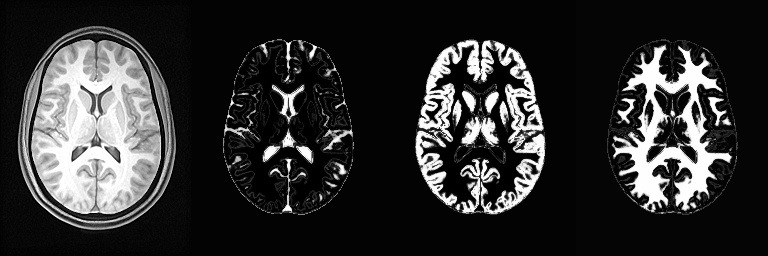
\includegraphics[width=0.9\textwidth]{templatefig.jpg} 
\itkcaption[Template Prior]{An example template.}
\vspace{-0.1in}
\label{fig:template}
\end{figure}

\section{Run a Cross-Sectional Study}
To run a pipedream study, your data needs to be organized as above and you need a template 
with all the necessary prior information available.  When all is ready, you will call:
\begin{verbatim}
    sh $PIPEDREAMDIR/pipedreamMapT1.sh pipedreamMapT1paramsUser.sh 
\end{verbatim}
where you likely have copied the ``base'' pipedreamMapT1paramsUser.sh
to your local directory and edited it for your data.  The output
directory structure and naming will mirror your input structure.  You
will get cortical thickness images, brain extraction, probability
maps, estimates of brain volume and---if enabled---a cortical
parcellation.

The key to the study is the file pipedreamMapT1paramsUser.sh.  
Within that file is a series of directory and then file variables that you need to define.  
We've tried to ``check'' your definitions for you and provide a warning that will help you 
find a mistake but this may not always work.  So, take care when making these definitions.

An important part of this step is how you distribute these processes.
We provide hooks for voxbo and for the SGE qsub.  There is also a
PIPEDREAMISTEST variable in the user configuration file that will set
``fast'' parameters to allow you to check your configuration before
running the full dataset.  Set variable GOTOVBQ=1, GOTOSGEQ=0 (for
voxbo) GOTOVBQ=0, GOTOSGEQ=1 (for sge) in pipedreamMapT1paramsUser.sh.  
If both are zero, you will run in serial mode. 

\section{Check Results}

Pipedream output is organized by subject and time point in a similar way to the input data, except that structural and DTI data are placed in the same directory. Within each time point output directory, there are the following files, prefixed with the subject ID and time point ID.

Images suffixed with ``norm.nii.gz" are normalized to standard space. If a mapping from the local template to standard space is provided, then all ``norm.nii.gz" are in standard space. Otherwise they are in the local template space. The images relating to DT processing are only produced if you have DT data for the subject and time point.

\begin{table}[htdp]
\caption{default}
\begin{center}
\begin{tabular}{| p{5cm} | p{10cm} |}
\hline
\textbf{Output} & \textbf{Description} \\ \hline
Affine.txt, InverseWarp.nii.gz, Warp.nii.gz & Warps from subject T1 to local template space. \\ \hline
brain.nii.gz & The brain-extracted and bias-corrected T1 image in subject space. \\ \hline
brainmask.nii.gz & The brain mask of the T1 image, used to compute brain.nii.gz. \\ \hline
brain\_prob\_[0,1,2].nii.gz & Segmentation probabilities of CSF (0), gray matter (1) and white matter in the T1 image. \\ \hline
deformed.nii.gz & Input head image deformed to the local template space. Useful for evaluating brain extraction and registration. \\ \hline
distcorr[Affine.txt, Warp.nii.gz, InverseWarp.nii.gz] & Distortion correction between T1 and DT space.\\ \hline
DTdeformed.nii.gz & DT image warped to the local template space \\ \hline
fa.nii.gz & Fractional anisotropy from DTI, in the subject space. \\ \hline
fadeformed.nii.gz & FA deformed into the local template space. \\ \hline
gmpnorm.nii.gz         & Normalized gray matter probability (brain\_prob\_1.nii.gz). \\ \hline
grid.nii.gz & Deformation grid showing the warp of the T1 image to template space. Used for evaluating registration. \\ \hline
head.nii.gz & Input T1 image. \\ \hline
kappa.nii.gz               & White matter curvature. \\ \hline
kappanorm.nii.gz   & kappa transformed to standard space. \\ \hline
logjacobian.nii.gz   & Log determinant of the Jacobian, in the local template space. \\ \hline
seg.nii.gz      & Three tissue segmentation of the T1 brain image.\\ \hline
thickness.nii.gz & Cortical thickness in the subject space. \\ \hline
thicknorm.nii.gz & Thickness warped to standard space. \\ \hline
\end{tabular}
\end{center}
\label{pipedreamMapT1out}
\caption{Output of pipedreamMapT1}
\end{table}%

If you have defined label images in the template space, there will be additional output containing the labels and probabilities in the subject space.

It's critical to evaluate the output data visually before doing statistics. The normalized images can be evaluated by extracting the same slice from all subjects, using ANTS:
\begin{verbatim}
    $ANTSPATH/StackSlices vol.nii.gz -1 -1 80  PipeDreamOutDir/*/*/*_thickness.nii.gz
\end{verbatim}
This will extract the 80th z-slice of every image and put it into a volume (vol.nii.gz) 
that you can scroll through.  You can call this on any image type.  If some specific dataset, e.g. subject00X, does not work, you 
may want to manually set the variable PIPEDREAMSUBJECTSLIST=subject00X and run a test 
on that subject alone, without sending to distributed computing, to see what is going on.  As above, if you 
set PIPEDREAMISTEST=1 you can get a fast test result for this subject.  

\section{Compute Statistics} 
If everything is good, you are ready to estimate group statistics.  We
prefer a {\bf R} statistical interface and can provide a script for
you.  However, you may run your favorite statistical package on the
output of pipedream.

\begin{comment}
\section{The PipeDream Preprocessing Pipeline} 
\subsection{Data Organization}
\subsection{T1 Pipeline} 
\subsection{DTI Pipeline}
\subsection{Quality Assurance}

\section{The PipeDream Cross-sectional Pipeline}

\subsection{The Importance of the Template}
\subsection{Customization}
\subsection{Required Software}

\section{The PipeDream Longitudinal Pipeline}

\section{A Working Example}
\subsection{The Template}
\subsection{The Data}
\subsection{The Results}
\subsection{The Longitudinal Results}
\end{comment}

\section{Annotated Bibliography}
The original statement of the symmetric normalization and template
construction methodology was given in \cite{Avants2004}.  A follow up
study that used landmark guidance to compare the chimpanzee cortex to
the human cortex was published here \cite{Avants2006} -- this study
used {\em in vivo} MRI and template-based normalization to confirm
volumetric numbers derived from an early 20th century post-mortem
study comparing one human and one chimp.  This conference article has
some additional detail and alternative updates to the methodology, in
particular application to shape-based interpolation
\cite{Avants2005b}.  Network based studies were performed here
\cite{duda08miccai,duda08cvpr}.  The main SyN paper is here
\cite{Avants2008}.  Applications to neurodegeneration are here
\cite{Avants2005,Avants2008a,Grossman2008,Avants2009,Das2009,Yushkevich2009,Massimo2009}.
Hippocampus focused work is here \cite{Pluta2009,Yushkevich2009}.  The
main evaluation papers include \cite{Avants2008} and \cite{Klein2009}
for the cortex and deep brain structures whereas \cite{Pluta2009}
evaluates the use of automated and semi-automated normalization for
high-throughput hippocampus morphometry.  An additional evaluation
paper is being developed.  


%%%%%%%%%%%%%%%%%%%%%%%%%%%%%%%%%%%%%%%%%
%
%  Insert the bibliography using BibTeX
%
%%%%%%%%%%%%%%%%%%%%%%%%%%%%%%%%%%%%%%%%%

\bibliographystyle{plain}
\bibliography{references,ants}


\end{document}

